\chapter{Project Overview}

\section{Introduction}

Our group is seeking to develop a reinforcement learning agent to support portfolio 
management and optimization. Utilizing both empirical stock pricing data along with 
alternative data, we look to create a more well-informed portfolio optimization tool. 

Our primary motivations for pursuing a reinforcement learning-based approach are as 
follows:

\begin{enumerate}
    \item Reinforcement learning lends itself well to learning/opening in an online environment. The agent can interact with its environment, providing real-time feedback/ responsiveness to allow for better results.
    \item Our approach involves incorporating alternative data to support the agent’s decision making process. Encoding this data the states matrix of the agent could allow for the agent to make better decisions when it comes to adjusting portfolio weights.
    \item Given that a reinforcement learning agent’s decisions are modeled by a Markov Decision Process, we can easily provide different reward functions to account for a variety of investor preferences or restrictions.
\end{enumerate}



\section{Dataset Creation}

Creating a textual corpus sufficient for us to build 
a robust reinforcement learning agent required us to pull and combine stock price data with SEC filings and news data. 
The proceeding section gives motivates our usage for each type of data we use and explains our data cleaning process.

\subsection{Stock Data}

We retrieve data from Wharton Research Data Services 
(WRDS). WRDS is a pre-eminent source of financial data that we have experience 
utilizing in the Computational Finance program’s other courses. Specifically, we want to utilize data from the Center for Research in 
Security Prices (CRSP), which has security price, return, and volume data for stocks listed in the 
NYSE, AMEX and NASDAQ exchanges. We created a our trading universe with the S$\&$P 100 stocks. 
For this dataset, limited cleaning was required and we discuss how it is incorporated into the states matrix in Section 1.3.

\subsection{News Data}

An important direction of our research is to explore how the performance 
of reinforcement learning trading agents are influenced by news data.
We believe that news data will impart an external understanding of how 
well a given stock is performing. Further, it could inform our agent on a stock's exposure market or sector risks. 
This could provide our agent a better view of the trading environment, which 
can help it make better decisions to maximize the reward. 

We initially attempted to query data from news APIs to get a more expansive news corpus. However, we found that due to the cost of obtaining the data, the computational power needed to process the headlines, and the storage needed to manage all of the data, that this would not be a feasible pursuit.

The dataset we use in this project is Daily Financial News for 6000+ Stocks that was downloaded via kaggle \cite{financial_news}.
This dataset contains scraped headline data for over 6000 stocks listed on the NYSE exchange from 2009-2020. 
There are two main files within this dataset that we use. The first is \texttt{raw\_analyst\_ratings.csv}, which only contains scraped data from a prominent financial news publisher Benzinga.
The other file \texttt{raw\_partner\_headlines.csv} contains scraped headline data from other smaller publishers that partner with Benzinga. Each row of the datasets contains a headline, the base article URL, the date and time of publication, and the stock ticker symbol.
The \texttt{raw\_analyst\_ratings.csv} file does not contain publisher information, as it is already implied that Benzinga is the publisher. Meanwhile, the table in \texttt{raw\_partner\_headlines.csv} has a column indicating the publisher of each article. 
We concatenate the headline data from each file to create a single unified dataset that contains all headlines for each stock in our universe.


\subsubsection{SEC Filings}\label{filings}

To enrich our dataset, we utilize SEC filings data for each of the S$\&$P100 companies. 
These filings contain essential information regarding a company's financial 
performance, governance, and compliance that could enhance our measure of 
company outlook. Specifically we aim to use data from 10-K and 10-Q filings. 
10-K filings are an annual report on a company’s performance, and include information. 
They are divided into items that show a company’s financial statements, 
stock projections, and pertinent information for shareholders in sections that 
are denoted as items. 10-Q filings are similar to 10-K filings, with the key differences being less detail given the quarterly frequency, along with unaudited financial statements.


\subsection{Sentiment Analysis}

Using the news sources and SEC filings data described above, we wish to 
generate embeddings from which we can extract sentiment related features 
to provide to our reinforcement learning agent. Our approach, which is to utilize the pre-trained 
FinBERT model, fine-tuned to recognize the sentiment of financial text to 
create embeddings for us \cite{finbert}. 

\subsubsection{FinBERT Sentiment Scores}\label{finbert}

Over the full trading period (2010-2020), we will feed all of the headlines and selected SEC filings text for S$\&P$ 100 companies to pre-trained FinBERT. 
The model then generates probabilities of the content having a positive, negative, or neutral sentiment. For the news headlines, we developed a novel function to extract a single embedding for a stock on a given day. 

The function that we created is:
\[\texttt{Value}_{\texttt{Embedding}} = \tanh\Biggl( \frac{\frac{\texttt{positive sentiment probability}}{\texttt{negative sentiment probability}}}{\texttt{neutral sentiment probability}} \Biggr)\]
This approach combines the “log likelihood” (ratio of probabilities of positive and 
negative sentiment) along with a penalty for high neutral sentiment (a measure of 
uncertainty), using the tanh for normalization. This approach would allow us to 
adequately detect strong positive/negative sentiment. Thus, a sentiment score close to 1 can be interpreted as a positive sentiment, a score close to 0 can be interpreted as neutral, and a score close to -1 can be intepreted as negative.

An issue that we run into when incorporating SEC filings data is that they are recorded on a annual or quarterly basis, which is far more infrequent than our samples for price and news data.
Thus, to fill the gaps between SEC filings dates, we apply exponential decay to the sentiment scores on report dates. Formally,

$$
y = a(1 - \gamma)^t
$$

Where $a$ represents the company's sentiment score on the reporting date, $t$ represents time (in days) between the last report date and the current day, and $\gamma$ is a constant between 0 and 1 representing the daily decay factor. We test $\lambda = 0.1, 0.5, 0.9$ in our models to see what performs optimally. Note that we test a wide range of $\gamma$ values because we are unsure of how fast the signal from SEC filings decay. We also run experimented with using this same routine to fill some gaps between news data.
 
\subsection{Finalized Data Processing Pipeline}
We dedicate this section of the paper to outline the pre-processing pipeline for both our SEC filings and news data.

\subsubsection{Creating News Tensors}\label{newstensors}

From the concatenated dataset of news headline data from each publisher as described in the "News Data" section, we feed the dataset (loaded into a pandas dataframe) through a multi-stage pipeline. 
The first step is to scrape the current $S\&P$ 100 companies and then filter the dataset down to only include headlines from companies in the $S\&P$ 100. 
We introduce a custom dataset class called "NewsHeadlines," implemented in PyTorch framework, designed for efficiently handling news headline data. 
The class takes a dataset and a user-defined tokenizer which will pre-process headlines in batches to be fed into FinBERT. 
In the class, we implement an iterator function \texttt{\_getitem}, which takes the raw headline data as input and returns an encoding for the batch of headlines after tokenization. 
Then given the large size of the dataset, we use a create a "Dataloader" object, implemented in PyTorch, which feeds our dataset into the model in small batches. 

To obtain the output tensors corresponding to the sentiment probabilities, we iterate over the batches, applying FinBERT to classify each headline and from the raw logits using the softmax activation function to a vector of probabilities.
Then for each batch, we save off the tensors to separate files. A finalized version of this process is available in \texttt{utilities\\news\_data\_processing.py}
Then in the \texttt{tensor\_data\_loading.ipynb} script, we merge the tensors with the original concatenated dataset and create our the sentiment embedding as described in the "FinBERT Sentiment Scores" section. 
This finalized dataset is then written to \texttt{news\_sentiment\_data.csv}

\subsubsection{News Dataset Statistics}\label{newsstats}

Our dataset contains data for 84 out of the total 100 tickers in the $S\&P$ 100, and it contains 70,872 entries containing the sentiment embedding of news for a company on a given day. Below are some reported summary statistics on the distribution of news reports across the tickers:

\begin{table}[htbp]
    \centering
    \caption{Company News Reporting Date Distribution}
    \begin{tabular}{l c}
        \toprule
        \textbf{Statistic} & \textbf{Value} \\
        \midrule
        Count & 84 \\
        Mean No. of Reporting Dates & 843.714 \\
        Standard Deviation & 508.209 \\
        Minimum Observations & 1 \\
        25th Percentile & 393.250 \\
        Median & 905.000 \\
        75th Percentile & 1198.500 \\
        Maximum & 1829 \\
        \bottomrule
    \end{tabular}
\end{table}

Note that given our median ticker only has news reports on 905 of the total trading dates and because there are 16 tickers for which we have no sentiment data, our dataset is still suboptimal for developing an agent. Our forward filling process, does address some of the gaps in our data, however our coverage is still not complete.
This is an important consideration when examining the results of our work.

Now, we will examine the distribution of sentiment scores across the articles to examine key facts about their distribution.


\begin{figure}
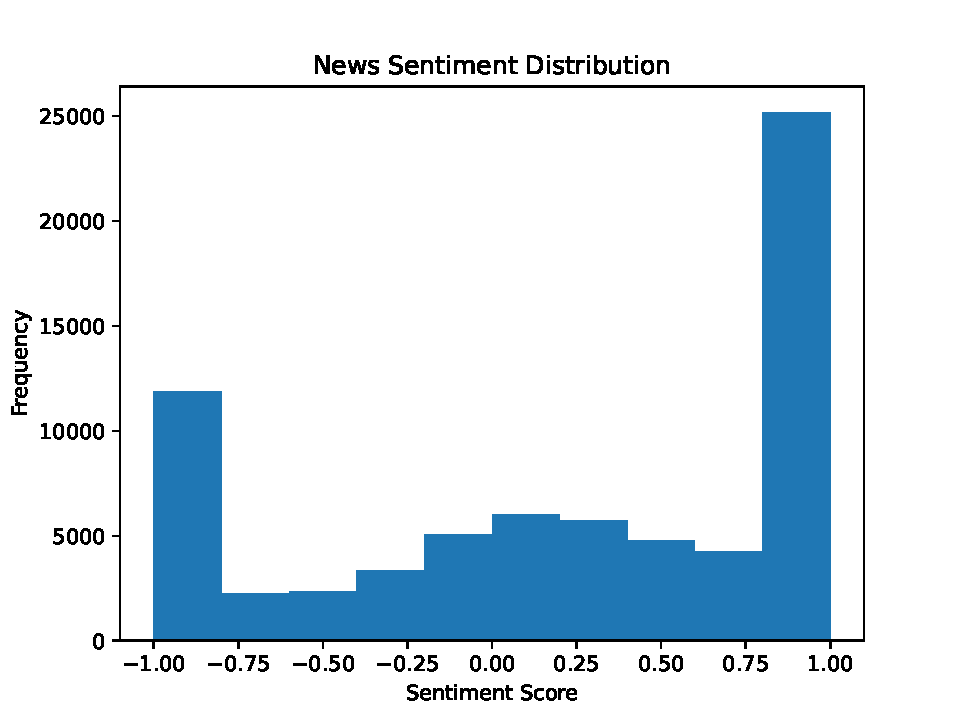
\includegraphics[width=.9\textwidth]{news_sent_dist}
\end{figure}

The figure highlights that news sentiment has a bimodal distribution. Much of the headlines are interpreted as either negative or positive, but news headlines that are relatively neutral, or closer to 0, or more evenly distriubuted. 
This indicates that the headlines that display strong enough sentiment that they could inform and change the actions of our reinforcement learning agents.

\subsubsection{Creating SEC Tensors}
To create tensors, we initially attempted to scrape the SEC's EDGAR database for all 10-K and 10-Q filings in the database's history, ranging from 1994 through 2023. The filings from the EDGAR database are returned as HTML files which we stored in a cloud database. The size of this database is roughly 108.3 GiB, or 116.3 GB.\\
To extract meaningful values from the text, we first parse and clean the HTML so we can extract the raw text from each document. Then we use regular-expression based text parsing to extract text from Item 1A and 7/7A, and Item 2 in 10-Qs. We then construct a data frame, where each row contains the company ticker, the date of the filing, the extracted section name, the text of the extracted section. We then pass this into the FinBERT model to add a final column containing sentiment scores, calculated by the methodology explained in Section \ref{finbert}. However, issues were encountered both with the size of the dataset being computationally intensive, along with parsing issues due to the way the filings are stored and transmitted.
The process to create SEC-sourced tensors is then to extract positive, negative, and neutral words as specified by the Loughran-McDonald sentiment dictionary. We then utilize the proportions in a similar fashion to the news embeddings:
\[\texttt{Value}_{\texttt{Embedding}} = \tanh\Biggl( \frac{\frac{\texttt{positive word count proportion}}{\texttt{negative word count proportion}}}{\texttt{neutral word count proportion}} \Biggr)\]
\subsubsection{SEC Filings Dataset Statistics}
Our dataset contains data for 99 out of the 100 tickers in the $S\&P$ 100, containing over 9,000 filings between 1994 and the present day, with the used subset consists of roughly 6,100 filings. Below are some reported summary statistics on the distribution of SEC filings across the tickers:

\begin{table}[htbp]
    \centering
    \caption{Company SEC Filings Distribution}
    \begin{tabular}{l c}
        \toprule
        \textbf{Statistic} & \textbf{Value} \\
        \midrule
        Count & 99 \\
        Mean No. of Filings & 61.42 \\
        Standard Deviation & 10.18 \\
        Minimum Observations & 20 \\
        25th Percentile & 64 \\
        Median & 65 \\
        75th Percentile & 65 \\
        Maximum & 66 \\
        \bottomrule
    \end{tabular}
\end{table}
Since there are only 4 filings per year, we use forward filling with decay to fill in the "missing" dates. Giving the addition and dropping of companies from the S&P100, as well as some newer public companies joining, each company does not have the same number of filings over the time period.\\
We now look at the distribution of sentiment scores as calculated in Section \ref{newsstats}:

\begin{figure}[H]
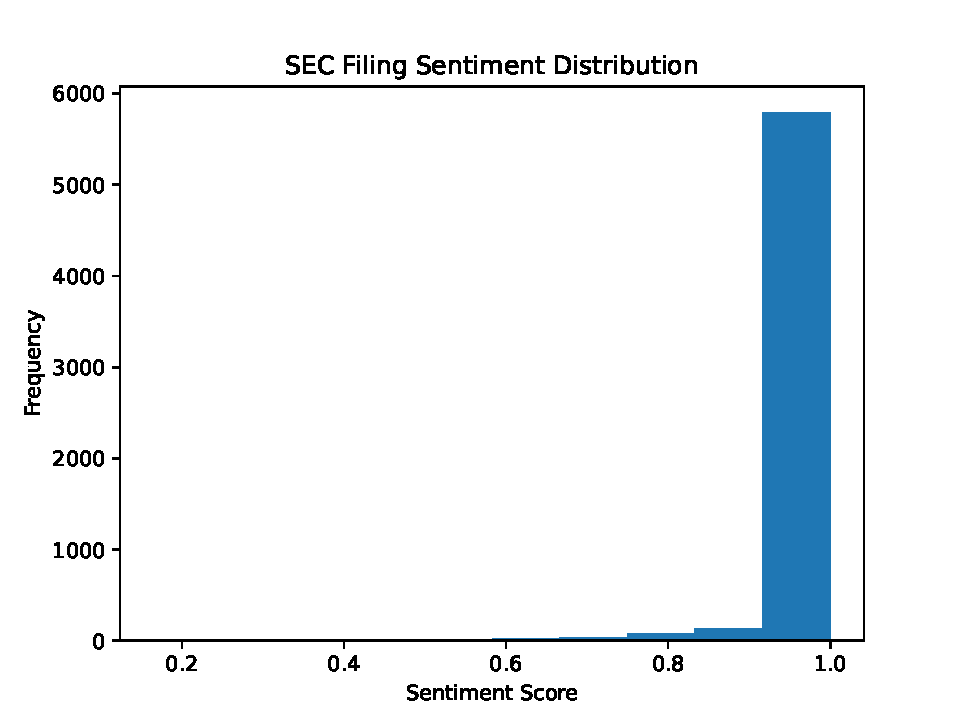
\includegraphics[width=.9\textwidth]{sec_sent_dist}
\end{figure}

There is a pronounced tail towards 1, indicating a strongly positive unimodal distribution, as compared to that of the news sentiment. Since we utilize sections of the SEC filings that are written by the companies themselves, it is likely that companies aim to provide filings that suggest strong performance and future outlook. In the dataset, we do observe some drops in sentiment, such as times of financial crisis or bad market conditions, like in 2013 for some technology-based companies.

\section{Algorithmic and Analytical Challenge}

Our primary model technique is deep reinforcement learning, which is a 
branch of machine learning that operates in a game-theoretic-like system. 
Formally, a reinforcement learning problem is an instance of a Markov 
Decision Process, which is a 4-tuple $(S, A, T, R)$: $S$ the state space 
(matrix of selected historical stock price and news data available to 
our model at a given time; see Methodology section), $A$ the action space 
(portfolio weights produced by our model, under appropriate constraints), 
$T$ the transition function (how the state changes over time, modeled by our dataset), 
and $R$ (the reward function). The goal is to find a policy (function from $S \to A$) 
that maximizes future expected rewards. Most reinforcement learning research is 
spent on providing good information in $S$ to the model, defining a good reward 
function $R$, and deciding on a deep learning model training system to optimize rewards.

\subsection{Existing Literature}

Much of the literature applying RL to portfolio optimization has arisen in the 
last few years. Some relevant papers are:

\begin{itemize}

\item \cite{drl_mvo} Deep Reinforcement Learning Comparison with Mean-Variance Optimization: 
Using a lookback of recent past returns and a few market indicators 
(including 20-day volatility and the VIX), this paper implements a simple 
algorithm for portfolio weight selection to maximize the Differential Sharpe Ratio, 
a (local stepwise) reward function which approximates (global) Sharpe Ratio of the 
final strategy. They compare their model with the standard mean-variance 
optimization across several metrics.

\item \cite{drl_modern_portfolio_theory} DRL for Stock Portfolio Optimization Connected with Modern 
Portfolio Theory: This paper applies reinforcement learning methods to 
tensors of technical indicators and covariance matrices between stocks. 
After tensor feature extraction using 3D convolutions and tensor decompositions, 
the DDPG method is used to train the neural network policy, and the algorithm 
is backtested and compared against related methods.
 
\item \cite{rl_augmented_states} RL-Based Portfolio Management with Augmented Asset Movement Prediction 
States: The authors propose a method to augment the state space S of historical 
price data with embeddings of internal information and alternative data. 
For all assets at all times, the authors use an LSTM to predict the price movement,
which is integrated into S. When news article data is available, different NLP methods 
are used to embed the news; this embedding is fed into an HAN to predict price 
movement, which is also integrated into S for state augmentation. The paper applies 
the DPG policy training method and compares against multiple baseline portfolios on 
multiple asset classes. It also addresses challenges due to environment uncertainty, 
sparsity, and news correlations.

\item \cite{drl_framework} A Deep Reinforcement Learning Framework for the Financial Portfolio Management Problem: 
This paper contains a deep mathematical and algorithmic discussion of how to properly incorporate 
transaction costs into an RL model. The authors also have a GitHub with implementations of their 
RL strategy compared with several others.

\item \cite{learn_to_rank} Stock Portfolio Selection Using Learning-to-Rank Algorithms with News Sentiment: 
After developing news sentiment indicators including shock and trends, this paper applies 
multiple learning-to-rank algorithms and constructs an automated trading system with strong performance.

\item \cite{maps} MAPS: Multi-agent Reinforcement Learning-based Portfolio Management System: 
This paper takes advantage of reinforcement learning with multiple agents by defining a 
reward function to penalize correlations between agents, thereby producing multiple orthogonal 
(diverse) high-performing portfolios.

\end{itemize}

\subsection{Methodology}

We will be implementing, combining, and improving on the methodologies of several of the above papers. 
Our plan is to develop an RL system that utilizes multiple time periods to achieve strong out-of-sample 
trading performance. As of this writing, we have partial implementations of papers \cite{drl_mvo}, \cite{drl_modern_portfolio_theory}, and \cite{drl_framework}.
 Our final architecture will be most similar to papers \cite{rl_augmented_states} and \cite{drl_framework}.

\subsubsection{Markov Decision Process Problem Formulation}

Paper \cite{rl_augmented_states} includes the following diagram, which is very close to our desired 
architecture:

\begin{center}
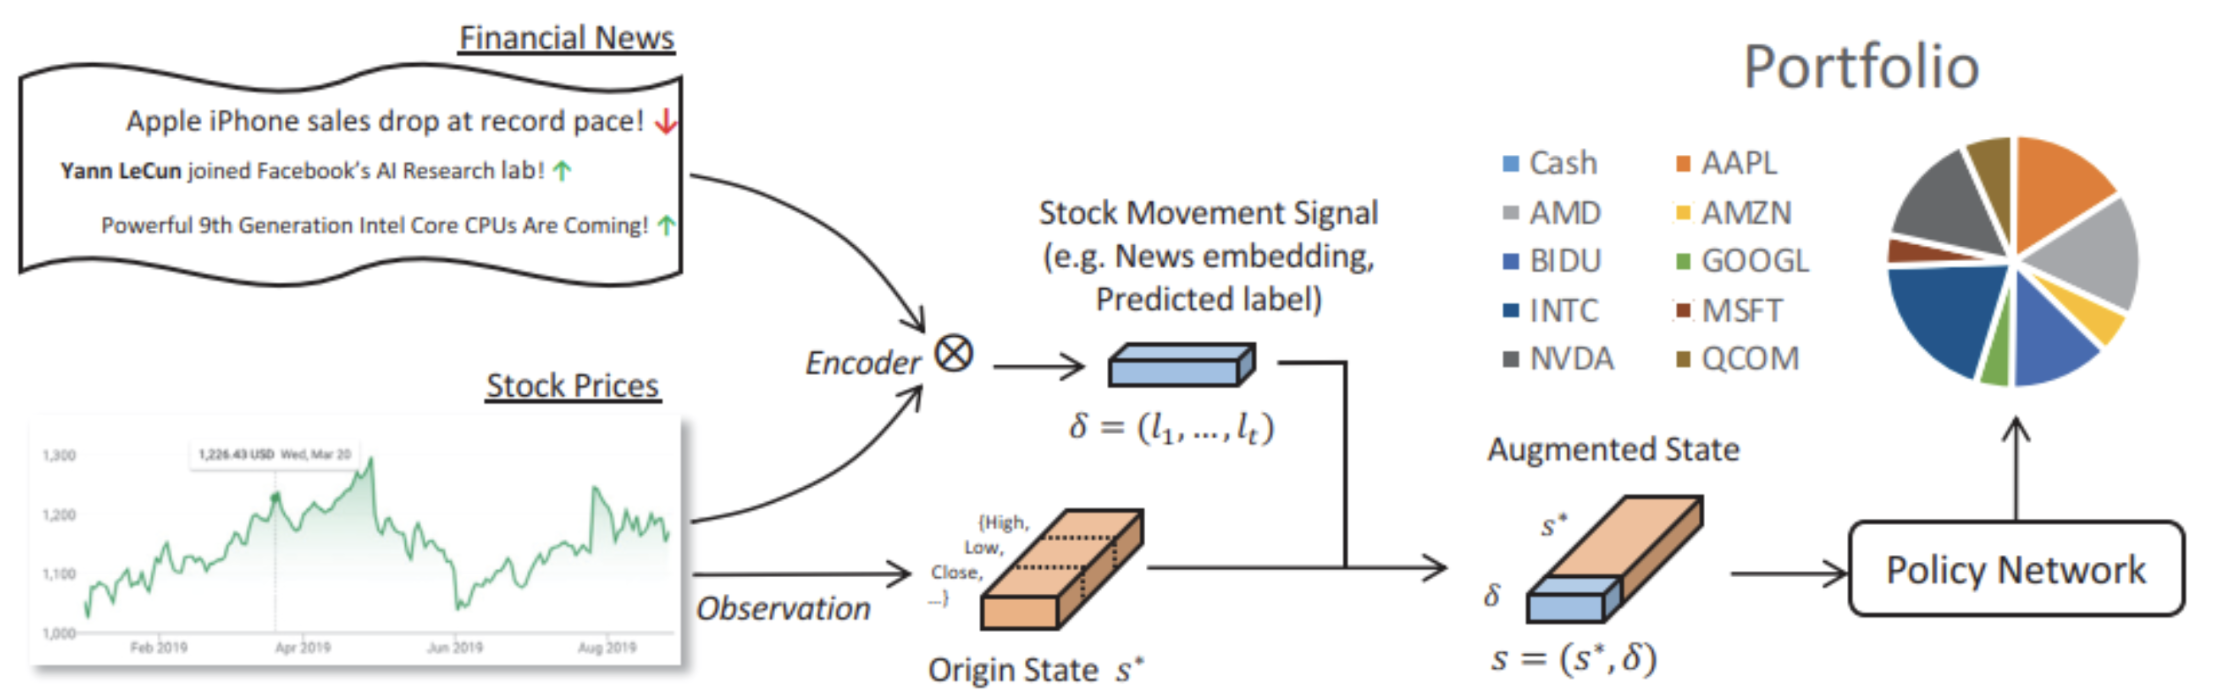
\includegraphics[width=13cm]{formulation.png}
\end{center}

An explanation of this diagram: at time t, the origin state $S^*$ is a 3D tensor of dimensions $U \times H \times C$
which contains historical price data. $U$ is the size of our universe (for example, for the S$\&$P100, $U = 100$). 
$H$ is the size of history we are providing (if we are providing 30 day history, then $H = 30$). 
$C$ is a categorical value representing the close/high/low price. This format of $S^*$ allows us to store, 
for example, the last 30 days of stock price data for all companies in the S$\&$P100, for any given day. 
In addition to this, we have news information $\delta$, obtained from financial news headlines for that day, 
processed through a pre-trained encoder. This information is added to $S^*$ to create the full state 
$S = (S^*, \delta)$

In our architecture, for $S^*$, we will experiment with the lookback period size and likely reduce it 
to a 2D array by flattening along the C index, but will otherwise keep $S^*$ largely the same. For 
$\delta$, we plan to utilize better feature extraction via sentiment scores and topic modeling; 
we also plan to use different alternative data sources, as described in the Dataset Creation section. 
In addition, we will extract what company each headline refers to, so our features can be changed 
over time independently for each company as news articles enter through our environment. The final 
state S will likely be a 2D matrix, where each row represents a different company (ticker), and along 
that row we find, concatenated, the following: (1) the past month-or-so of stock price data from $S^*$, 
and (2) numerical features extracted from recent news data pertinent to that company (as described 
in the Dataset section). (The straightforward concatenation of price data and news embeddings did not 
affect the ability of the neural network-based agent to learn.)

Regarding the reward function R, we plan to experiment with both the profit reward function used in \cite{rl_augmented_states}, 
as well as the Differential Sharpe Ratio developed in paper \cite{drl_mvo}.

In summary, our project aims to implement and replicate the approach used in \cite{rl_augmented_states}, with 
some modifications to S and R as previously described. We will conduct experiments alternative data 
sources, feature extraction methods, and reward functions (both custom and from other papers listed) 
to find a good combination that allows this approach to work well on S$\&$P100 stocks; this comprises our 
novel extension/contribution.

\subsubsection{Use of Libraries}

We will mainly be using the Gymnasium library to implement the reinforcement learning environments. 
The Stable Baselines 3 library provides several policy learning techniques that we will experiment with, 
including Proximal Policy Optimization (PPO) and Deep Deterministic Policy Gradients (DDPG). 
The papers above discuss the advantages and disadvantages of multiple reward functions and constraints, 
which we will make improvements upon and provide as options to the user, if applicable.

\subsubsection{Strategy Benchmarking}

Our final model architecture will be compared against several benchmark financial portfolio selection 
models. Among these will be the CAPM, an exponential moving average strategy, linear factor models 
such as the Fama French 3/5-factor models, and the QMJ model. We will compare our returns 
in-sample and out-of-sample plots, as well as our relative performance on portfolio statistics 
including cumulative return, Sharpe Ratio, Sortino Ratio, drawdown, etc. The experiment sections 
in the above papers provide a strong reference for our methodological comparison.

